\mysection[black]{4. Types}



\mysubsection{4.1 Lambda Calculus}
\textbf{Lambda Calculus}: \texttt{(fun x -> e)}, or $\lambda x.e$, turing complete 

 \begin{multicols}{2}
\textbf{Abstract Syntax}\\
\begin{lstlisting}
type exp =
| Var of var
| Fun of var * exp 
| App of exp * exp
\end{lstlisting}
\columnbreak

\textbf{Concrete Syntax}\\
\begin{lstlisting}
exp ::=
| x 
| fun x -> exp 
| exp1 exp2 
| ( exp )
\end{lstlisting}
\end{multicols}
\textbf{Application}: Interpreted by substitution {\scriptsize\texttt{(fun x -> fun y -> x + y) 1= subst 1 x (fun y -> x + y)= (fun y -> 1 + y)}}
\textbf{Substitute}: free $x$ with $y$ in $e$: \texttt{e\{y/x\}}, cases:
\begin{itemize}[leftmargin = *,noitemsep]

\item \textbf{Variable (matching):}  
\texttt{x\{v/x\} = v}.

\item \textbf{Variable (non-matching):}  
\texttt{y\{v/x\} = y} if $x \neq y$.

\item \textbf{Function (shadowing):}  
\texttt{(fun x -> exp)\{v/x\} = fun x -> exp}.

\item \textbf{Function (non-shadowing):}  
\texttt{(fun y -> exp)\{v/x\} = fun y -> exp\{v/x\}} if $x \neq y$.

\item \textbf{Application:}  
\texttt{(e$_1$ e$_2$)\{v/x\} = (e$_1$\{v/x\} e$_2$\{v/x\})}.
\end{itemize}

\textbf{Free/Bound:} In \texttt{fun }$\alpha$\texttt{ -> }$e$, an \emph{occurrence} of a variable $v$ is \emph{bound} if $v = \alpha$ and the occurrence appears in $e$; an occurrence of
$v$ is \emph{free} if $v \neq \alpha$, the occurrence appears in $e$, and it is
not bound by any enclosing \texttt{fun}.\\
\textbf{Capture Problem (CP)}: Naïve subst. is not sound  {\scriptsize\texttt{(fun x -> (x y)) \{(fun z -> x) / y\} = fun x -> (x (fun z -> x))}}\\
\textbf{Alpha-Equivalence}: Name of bound var. can be subst. $(\operatorname{fun} {\color{Aquamarine}x} \rightarrow y{\color{Aquamarine}x})\equiv (\operatorname{fun} {\color{Aquamarine}z} \rightarrow  y{\color{Aquamarine}z})$\\
\textbf{Sol. to CP}: In \texttt{e1\{e2/x\}} chose $\alpha$-equiv. s.t. the bound vars of $e_1$ don't mention the free vars of $e_2$, then subst.

\mysubsection{4.2 Typechecking}
\textbf{Type}: Predicate on the set of values in a system, abstraction mechanism 
\textbf{Inference Rule}: $\exp \Downarrow v$, program $\exp$ eval. to val. $v$\\
\textbf{Object- vs. Meta-level}: $+$ vs $\llbracket+\rrbracket$\\
\textbf{Proof-Tree}: Nudes are judgements, Edges connect premises to conclusions\\
\textbf{Type-Checker}: Verify existence of proof tree\\
\textbf{Type-Judgement}: $C \vdash e: t$, under typing context $C$, expr. $e$ has type $t$, judgement holds $\Leftrightarrow$ can be derived with proof tree\\

\textbf{Compilation}: Treats typing judgement as $\llbracket \mathrm{C} \vdash \mathrm{e}: \mathrm{t} \rrbracket=$ ty, operand, \textcolor{Aquamarine}{stream} with the invariant: After executing $\operatorname{instrs}$, the operand $\operatorname{op}$ contains the value of $e$ and has type $\operatorname{ty}$ i.e. $\llbracket C \vdash 341+5:$ int $\rrbracket=$ \texttt{(i64, \%tmp, \textcolor{Aquamarine}{[\% tmp = add i64 (Const 341) (Const 5)]})}\\
\textbf{$\llbracket C\rrbracket$}: Finite map from identifiers to ty. i.e. \texttt{x:int, y:bool}

\BDEF{Thm: Simply typed $\lambda$ calculus with int.}{$$
\text { If } \vdash e: t \text {, then there exists a value } v \text { such that } e \Downarrow v
$$}

\BDEF{Thm: Type-Safety}{
If $\vdash \mathrm{P}: \mathrm{t}$ is a well-typed program, then either
\begin{itemize}
    \item[(a)]  the program terminates in a well-defined way, or
    \item [(b)] the program continues computing forever
\end{itemize}
}
\textbf{Short-Circuit Eval.}: $\llbracket C \vdash \operatorname{false} : \operatorname{bool}@ \rrbracket \text{Itrue} \text{ Ifalse}$, directly return stream of appropriate branch, i.e. it returns a jump not a value

\textbf{Compiling first order Functions}: Strategies:
\begin{itemize}[leftmargin = *,noitemsep]
\item \textbf{Reify}: Replace meta-level substitution with explicit runtime environments and variable lookup.
\item \textbf{Closure Conversions}: Eliminate free variables by packaging code with an environment into closures.
\item \textbf{Hoisting}: Separate code from data by lifting closed function bodies to the top level.
\end{itemize}


\mysubsection{4.3 Mutability \& Subtyping}

\textbf{Subtyping Hierarchy}: Partial ordered set 
\begin{itemize}[leftmargin = *,noitemsep]
\item \textbf{Reflexive}: $T <: T$ for any Type $T$
\item \textbf{Transitive}: $T_1 <: T_2 \wedge T_2 <: T_3 \Rightarrow T_1 <: T_3$
\item \textbf{Antisymmetric}: $T_1 <: T_2 \wedge T_2 <: T_1 \Rightarrow T_1 = T_2$
\end{itemize}
\textbf{Soundness}: A subtyping rel. $T_1 <: T_2 $ is sound if it appr. the underlying
semantic subset relation $\llbracket \mathrm{T} \rrbracket=\{\mathrm{v} \mid \vdash \mathrm{v}: \mathrm{T}\}$\\
\textbf{THM}: If $T_1 <: T_2 $ implies $s \llbracket T_1 \rrbracket \subseteq \llbracket T_2 \rrbracket$, then $T_1<: T_2$ is sound i.e. $\operatorname{Pos} <: \operatorname{Int}$ is sound, since $\{1,2,3, \ldots\} \subseteq\{\ldots,-3,-2,-1,0,1,2,3, \ldots\}$\\
\textbf{LUB}: From sound subtyping relation it follows that: $\llbracket T_1 \rrbracket \cup \llbracket T_2 \rrbracket \subseteq \llbracket \operatorname{LUB}(T_1, T_2) \rrbracket$\\
\textbf{Downcasting}: If casting to sub-type is required i.e. from $\operatorname{int}$ to $\operatorname{pos}$, one can downcast. Result of $\operatorname{int}$ not known during compile-time. Checked Downcasting allows for branches where conditions hold. i.e. 

\begin{prooftree}  
\AxiomC{$E \vdash e_{1}: \operatorname{int}$}
\AxiomC{$E,x: \operatorname{Pos}\vdash e_{2}: T_{2}$}
\AxiomC{$E \vdash e_{3}: T_{3}$} 
 \TrinaryInfC{$E \vdash \operatorname{ifpos} (x = e_{1}) e_{2} \operatorname{else} e_{3}: T_{2}\vee T_{3}$} 
\end{prooftree} 

\textbf{Subtyping of Functions}: Make argument contra- and output covariant. 
\begin{prooftree} 
\AxiomC{$S_{1}<: T_{1}$} 
\AxiomC{$T_{2}<: S_{2}$} 
 \BinaryInfC{$(T_{1}\to T_2)<:(S_{1}\to S_2)$} 
\end{prooftree}

\textbf{Immutable Records}: Datastructure where  fields are fixed at creation time, used for type systems, functional programming, as they are safe \& predictable\\
\textbf{Projection}: Allows to select specific fields of a record i.e. $e:\{l_1 :T_1 , ...\}$ to $e.l_i : T_i$ \\
\textbf{Width Subtyping}: A record type with more fields is a subtype of a record type with fewer fields, as long as the shared fields have the same types. $m< n \Rightarrow \{l_1 : T_1, \ldots, l_n:T_n \}<: \{l_1 : T_1, \ldots, l_m:T_m\}$ A code expecting a subtype will only access known vars, thus only accessing shared ones, order of field matters\\
\textbf{Depth Subtyping}: A record type is a subtype if corresponding fields have more specific types. $T_1 <: U_1 , \ldots T_n <: U_n \Rightarrow \{l_1 : T_1 ; \ldots ; l_n : T_n\} <: \{l_1 : U_1 ; \ldots ; l_n : U_n\}$ A more specific value can be used when a more general value is expected.

\textbf{Both}: Width subtyping doesn't allow permutation, to implement both dictionary implementation is needed.

\textbf{Covariance}: $T<: U \Rightarrow C[T]<: C[U]$, where $C$ is a constructor
\textbf{Contravariance}: $T<: U \Rightarrow C[T] :> C[U]$
\textbf{Invariance}: Neither Co- nor Contravariance holds
\textbf{Mutable Structures}: Only type-safe if Invariant, writing leads to problems i.e. for both subtyping:
\begin{itemize}[leftmargin = *,noitemsep]
\item \textbf{Width}: \textcolor{Red}{EXAMPLE FERDINAND ????    }
\item \textbf{Depth}: $x:\operatorname{Pos}<: x: \operatorname{Int}$ and then we can set $x=-3$, which is allowed with $x: \operatorname{Int}$ but break type-safety since $x:\operatorname{Pos}$ 
\textbf{References}: Co- and Contravariant references are unsound. Counter example same as for general mutable objects

\end{itemize}


\textbf{Structural Type}: Compatible based on their structure (what fields and types they contain), not on their names.\\
\textbf{Nominal Type}: Compatible based on explicit declarations and names, not structure.

\textbf{Dispatch Problem}: Same interface implementable through different classes\\
\textbf{Dispatch Vector (DV)}: At runtime objects store pointer to Dispatch Vector, which contains pointers to actual function implementations. Synonym for virtual / v-table, assume \texttt{s.size()} is called, then 
\begin{enumerate}[leftmargin = *,noitemsep]
\item Load the object \texttt{s}
\item Read the dispatch vector pointer from the object
\item Jump to the function pointer at a fixed index (e.g. index 2 for \texttt{size})
\item Pass \texttt{s} as the implicit \texttt{this} argument
\end{enumerate}
\textbf{Indices of V-Table}: Subclasses reuse the same index for inherited methods, Overridden methods replace the function pointer at that index
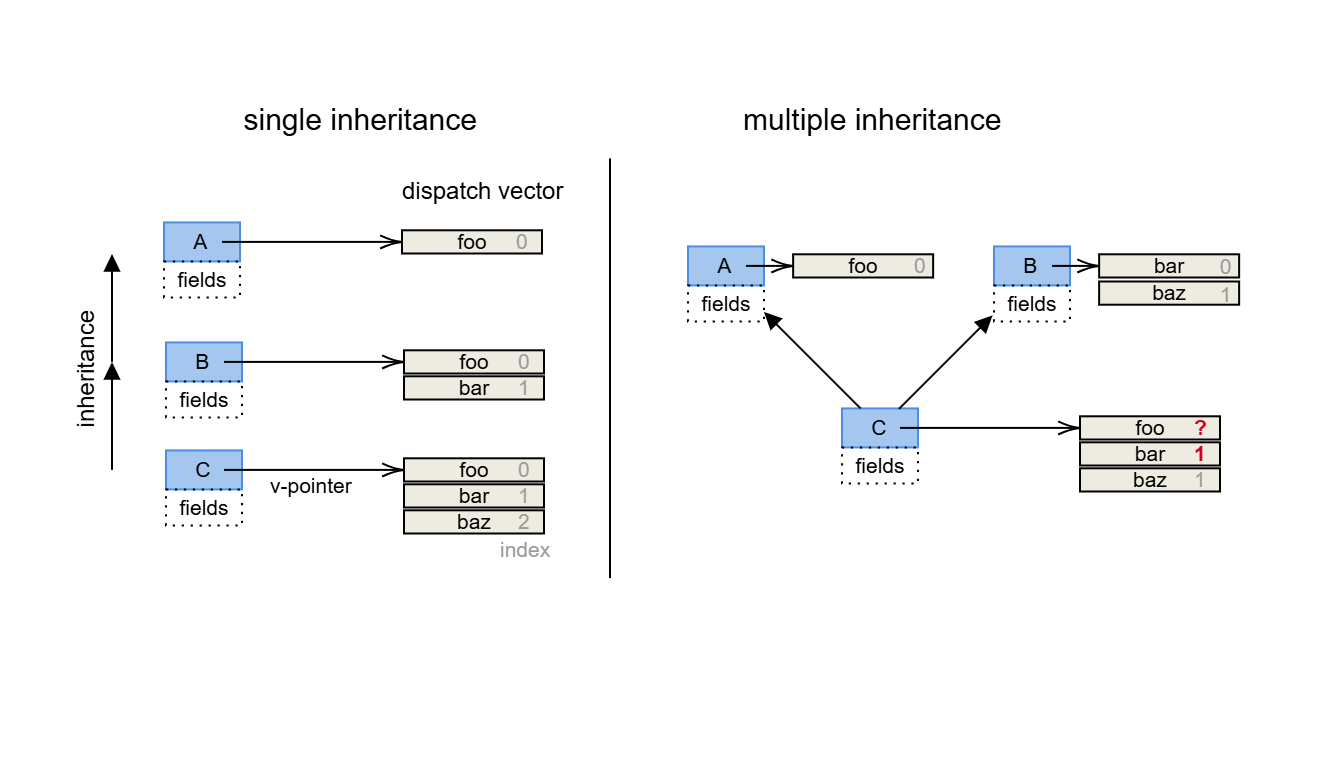
\includegraphics[width=1\linewidth]{images/inheritance.png}
\textbf{Solutions}
\begin{itemize}[leftmargin = *,noitemsep]
 \item One DV per superclass, calls use the dispatch vector corresponding to the static type at the call site. \textbf{Pros:} O(1), supports separate comp. \textbf{Cons:} Implicit casting, diamond inheritance doesn't work, \textbf{Procedure}: eval object, (\texttt{new C()}), get static type (\texttt{A x = new C()}), use v-ptr for type (\texttt{A}), used in c++
 \item Store class info structure, with pointer to superclass, mapping method-name to function pointer \textbf{Pros}: Caches optimize repeated calls to amortized O(1). Avoids index conflicts and supports multiple inheritance, \textbf{Cons}: Complex impl. \textbf{Procedure}: Look for f-name in class structure, if not found, move to superclass
 \item Every method is given global unique slot by compiler building inheritance graph, \textbf{Pros}: Fastest option, simple at runtime, \textbf{Cons}: No separate compl. possible, all code needs to be recompiled, different variants: Sparse DV Tables, Bin. Search Tree
 
 
 
 Compiler computes global method layouts using knowledge of the entire class hierarchy.
Each method gets a unique global slot; dispatch vectors may be sparse or replaced by decision structures. Enables fast dispatch with a single vptr, but breaks separate compilation and requires whole-program knowledge.
\end{itemize}

